\chapter{Introduction}
\label{ch:Introduction}

% what are we trying to solve / what is the problem?
% why is it important?

% minimize faulty material
% change contact pressure of steel belt rolls if something's going wrong
% cost reduction
% automatization (IoT, Industry 4.0)

% perform quality checks with sensors
% mechanical parameters can be calculated from magnetic field data
% highly sensitive MEMS gradient magnetometer
% try to predict faulty material in real time

Industry is ever-changing. Especially people working in the information technology branch know that, since these are the people that have to upgrade the current systems using latest technology. The latest industry-changing milestone was the rise of the so-called Industry 4.0, which combines regular mechanical processes with modern information and communication technology.

Industry 4.0 is a term that was coined by the German government \autocite{Industrie4.0Paper}. It describes the fourth industrial revolution. As explained in \citetitle{Industrie4.0History} the first industrial revolution took place around 1800 with the rise of steam and water-powered machines \autocite{Industrie4.0History}. One century later electricity heralded the start of the second industrial revolution, production lines being one of the biggest milestones. Also division of labour was first practiced. The third industrial revolution occurred with the invention of computers, robots and computer automation. The fourth and final one basically just refines the third revolution. This revolution includes the term \textit{cyber-physical systems}, which are systems that are controlled by computers, algorithms and sensors. This also means that there has to be some kind of communication between these systems which happens mostly over the internet. Figure \vref{fig:industry40} depicts this sequence of revolutions.

\begin{figure}[H]
    \centering
    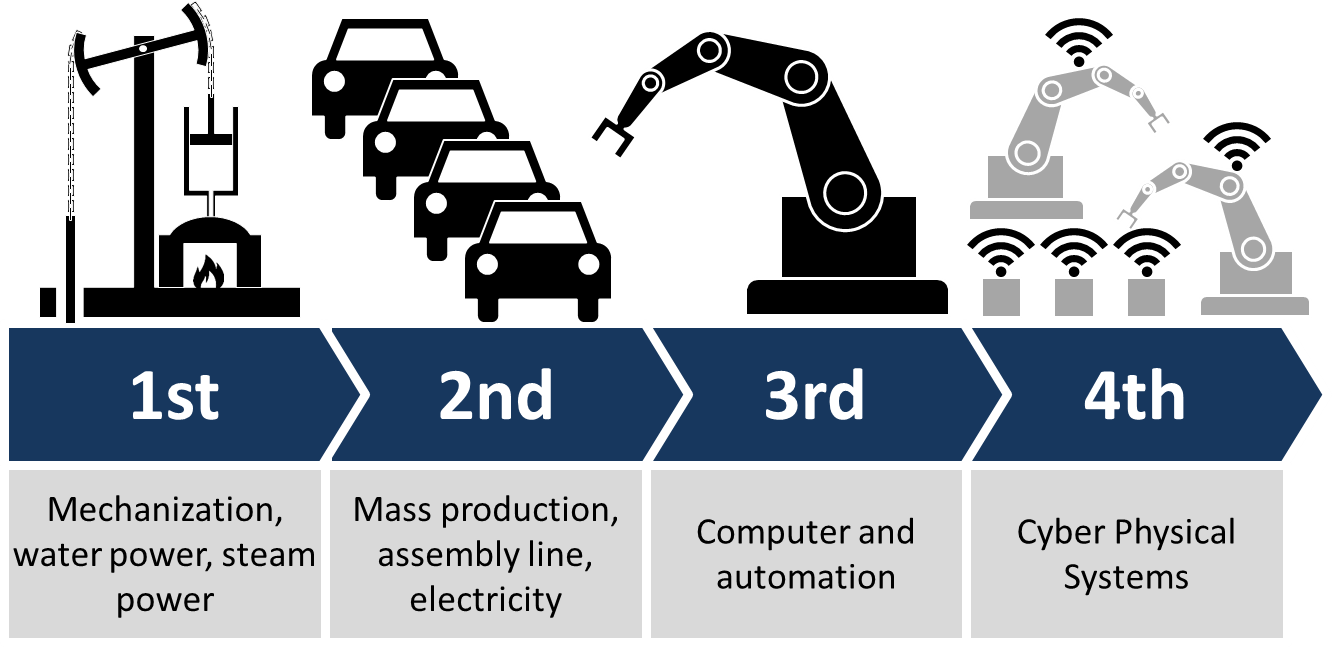
\includegraphics[width=11cm,keepaspectratio]{industry40}
    \caption[The four industrial revolutions that took place over the last centuries]{The four industrial revolutions that took place over the last centuries\footnotemark}
    \label{fig:industry40}
\end{figure}
\footnotetext{\cite{img:industry4.0}}

This drastic change means that many companies have to adapt. These adaptions had to be made to keep up with the competing companies that already have these technologies.

Steel belt production companies are no exception. With the invention of a gradient magnetometer that can effectively characterize steel belts, the foundation for this diploma thesis was laid.

\todo{cite patent?}

\section{Task}

The task of this diploma thesis is to develop a system to read sensor data, process it and visualize the results. Sensor data is continuously read from a highly sensitive MEMS gradient magnetometer. This data is structured as raw binary data and has to be processed by the system. The processed data will also undergo statistical analysis to predict parameters on the basis of this data. After this processing step the data has to be sent wirelessly to a mobile app. This mobile app acts as the client-side of the system. The app visualizes the sensor data and its predicted parameters. The app should also offer a way of browsing through historical data that was saved prior.

\subsection{Requirements of GRAMOC}
To achieve an efficient visualization of the extensive amounts of sensor data transmitted over network, GRAMOC needs to fulfill a certain list of requirements.

Server side requirements:

\begin{itemize}
    \item Read data from a sensor
    \item Save sensor data for further inspection
    \item Predict mechanical parameters from sensor data
    \item Send data to clients
    \item Provide historical data to clients
\end{itemize}

Client side requirements:

\begin{itemize}
    \item Visualize sensor data
    \item Provide a form for requesting historical data
    \item Visualize historical data
\end{itemize}

\section{Current Solutions}

\subsection{Existing Solution for Steel Belt Quality Inspection}

Currently there are no solutions for dynamic steel belt characterization. All these measurements have to be made manually.

The current procedure to inspect the quality of a steel belt is as follows: The first thing that has to be done is to produce a roll of steel belt. To get the quality level of this product, a sample has to be taken from it. There are two samples taken from each steel belt roll, one from the start and one from the end. These two samples can now undergo quality inspection procedures. The results from these tests can be used to assess the produced steel belt. According to these tests, the parameters of the production machines can be adjusted.

This procedure has a few major disadvantages. Firstly, if the product does not pass the quality tests, the whole steel belt has to be discarded. Time and personnel are also two big disadvantages. These quality tests are not only time consuming but they also require special trained staff for conducting these inspections.

\subsection{Existing Solutions for Handling Sensor Data}

Currently there are a lot of solutions available that can plot sensor data. The majority of these is even free. The one constraint that most of these solutions share is that the sensor has to be directly connected to the computer. As the sensor that is used for this project sends its data over the network, almost all solutions are considered irrelevant. Also some custom features are wanted that these programs do not offer. For example visualizing historical data.

\subsection{Existing Solutions for Plotting Real Time Data}

As already mentioned there are a lot of solutions out there that can be used to plot sensor data. But the one thing that these solutions mostly can not provide is real time plotting. Static plots can be achieved in many different ways, with big amounts of data or just small amounts, many plots combined or divided in separate plots and many more variations are within the bounds of possibility. A lot of these solutions promote themselves with ``dynamic data updates'' or ``streaming data''. That just means that the data can be changed at runtime and therefore some could say the data is displayed in real time. But real time can be defined very differently. As one would say real time applications can update their data once every second, others consider that the data must be updated within less than 20 milliseconds to achieve a high framerate. Most of the solutions available can handle the former definition of real-time but nearly none of them can provide enough performance for the latter. Another important point is the amount of data that one wants to depict, because most of the already existing programs that can handle real-time are just powerful enough to handle small amounts of data.

\section{Outline}

This diploma thesis is structured into two big parts. These parts can be seen as two phases of implementation. Each phase is completely separate. The first phase is a more experimental one as both authors were unfamiliar with these types of projects, so some experience had to be made. At the end of this phase there was a big cut and the project was restarted from the beginning. The second phase discusses the different approaches and decisions that were made starting from this cut. The second phase was not only better planned, but the decisions that were made, were mostly made out of experience from the first phase.
